\section{Web-app amministratori}
\subsection{Introduzione}
La web app costituisce l'interfaccia tramite la quale l'amministratore può interagire col sistema.
Le funzionalità offerte sono:
\begin{itemize}
	\item login e logout;
	\item visualizzazione delle stanze e delle postazioni con i relativi stati;
	\item aggiunta, rimozione e modifica di stanze e postazioni;
	\item impostazione di postazioni come guaste;
	\item impostazione di stanze come inaccessibili;
	\item visualizzazione delle credenziali degli utenti;
	\item aggiunta, rimozione e modifica di credenziali;
	\item visualizzazione e scaricamento report sulle occupazioni e sulle igienizzazioni;
	\item visualizzazione di notifiche riguardanti il salvataggio dei dati sulla blockchain.
\end{itemize}

\subsection{Requisiti e installazione}

\subsubsection{Ottenimento codice}
I file sorgente della web app si trovano su GitHub all'indirizzo \url{https://github.com/DPCMGroup/bc19-webapp}. Essi si possono scaricare compressi in formato zip direttamente dal sito, oppure tramite il comando \newline
\texttt{git clone https://github.com/DPCMGroup/bc19-webapp} \newline
se si ha già installato il software di versionamento Git.

\subsubsection{Linguaggi}
\paragraph{Typescript}
Superset del linguaggio \glock{Javascript}. Viene utilizzato per definire la logica dell'applicazione. \newline
Per poterlo utilizzare con \glock{Angular}, esso va prima installato col comando \newline
	\texttt{npm install -g typescript}

\paragraph{HTML}
Linguaggio di markup utilizzato per definire la struttura delle pagine web. Non necessita di installazione.

\paragraph{CSS}
Linguaggio per la definizione dello stile grafico delle pagine web. Nella nostra applicazione il codice \glock{css} introdotto da noi è molto limitato perché, per questo, ci siamo affidati al \glock{framework} Bootstrap. CSS non necessita di installazione.

\subsubsection{Tecnologie}
\paragraph{Node.js}
Programma focalizzato sull'esecuzione di codice javascript al di fuori di un browser.
Per l'installazione fare riferimento alla pagina \url{https://nodejs.org/en/download/}. La versione utilizzata per lo sviluppo è la 10.24.0.
\paragraph{npm}
Acronimo di Node Package Manager, permette di ottenere le librerie necessarie allo sviluppo.
Si ottiene insieme a \glock{Node.js} tramite l'installazione di quest'ultimo. La versione utilizzata per lo sviluppo è la 7.6.2.
\paragraph{Angular}
Framework per applicazioni web.
Per l'installazione fare riferimento alla pagina \url{https://angular.io/guide/setup-local#install-the-angular-cli}. La versione utilizzata per lo sviluppo è la 11.2.7.
\paragraph{Bootstrap}
Framework per la creazione di pagine web.
Per l'integrazione di Bootstrap in Angular fare riferimento alla pagina \url{https://www.npmjs.com/package/@ng-bootstrap/ng-bootstrap#installation}. La versione utilizzata per lo sviluppo è la 4.5.0.

\subsubsection{Test}
Per i test abbiamo utilizzato il framework Jasmine. Per utilizzarlo con Angular è necessario installarlo col comando \newline
	\texttt{npm install -g jasmine} \newline
La versione di Jasmine utilizzata per lo sviluppo è la 2.8.0. \newline
Per eseguire i test usare il comando \newline
	\texttt{ng test} \newline
I test verranno eseguiti tramite il programma Karma e i loro risultati saranno visualizzati in una pagina del browser aperta automaticamente.

\subsubsection{Ambiente di sviluppo}
Per lo sviluppo abbiamo utilizzato l'IDE WebStorm. Per la sua installazione riferirsi alla pagina \url{https://www.jetbrains.com/webstorm/download/}. La versione utilizzata per lo sviluppo è la 2020.3.3.

\subsubsection{Esecuzione}
Una volta installate le tecnologie sopra elencate si potrà eseguire la webapp aprendo un terminale nella root del progetto ed eseguendo il comando \newline
	\texttt{ng serve} \newline
Verrà eseguito un server locale accessibile all'indirizzo \url{http://localhost:4200}


\subsection{Architettura}
L'architettura della web-app segue il modello a componenti imposto da Angular, che, a sua volta, si basa sul pattern Model-View-ViewModel, descritto dall'immagine sottostante.
\begin{figure}[H]
	\centering
	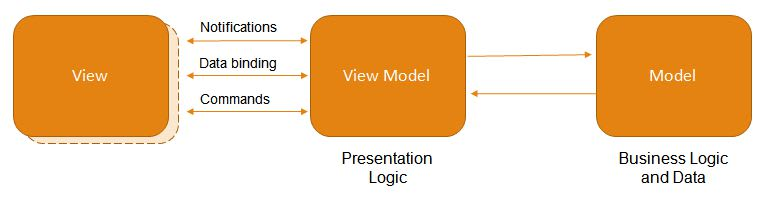
\includegraphics[width=15cm]{res/images/mvvm.jpg}
	\caption{Model-View-ViewModel}
	\label{fig:Model-View-ViewModel}
\end{figure}
Il modello imposto da Angular prevede che ogni funzionalità disponibile all'utente sia costituita da una vista (view) e da una logica (viewmodel) e chiama l'insieme di queste due parti "componente".
Gli attributi del componente sono accessibili alla vista. Questa caratteristica permette una sincronizzazione in due versi: la vista, per mano dell'utente, può modificare le variabili del view model, e se quest'ultimo modifica le proprie variabili, la vista si modifica di conseguenza.
Oltre ai componenti Angular offre la possibilità di creare dei servizi, che costituiscono la terza componente del pattern: il model. Questi servizi si occupano della gestione dei dati. Per esempio può esserci un servizio per la comunicazione col database, uno per la lettura e scrittura dal local storage e un altro che implementa un algoritmo per la manipolazione dei dati.
Un componente è costituito da 4 file. Nel seguente esempio è rappresentato un componente chiamato base.
\begin{verbatim}
	base.component.css
	base.component.html
	base.component.spec.ts
	base.component.ts
\end{verbatim}
I file contengono, nell'ordine:
\begin{itemize}
	\item lo stile grafico della vista del componente;
	\item la struttura della vista del componente;
	\item i test definiti per il componente;
	\item il codice che definisce la logica del componente.
\end{itemize}

I servizi sono definiti solo da due file. Di seguito sono mostrati i due file prendendo come esempio un servizio chiamato login. 
\begin{verbatim}
	login.service.spec.ts
	login.service.ts
\end{verbatim}
I file contengono, nell'ordine:
\begin{itemize}
	\item i test definiti per il servizio;
	\item il codice che definisce la logica del servizio.
\end{itemize}

La struttura del sito è definita principalmente dal modo in cui i componenti vengono annidati l'uno dentro all'altro. Nel codice \glock{html} questo annidamento è descritto dai tag:
\begin{itemize}
	\item \texttt{<app-nomecomponente>}
	\item \texttt{<router-outlet>}
\end{itemize}
In entrambi i casi, nella pagina visualizzata, verrà inserito il componente specificato al posto del tag. Nel primo caso il componente da inserire è fisso ed è definito dal nome del tag stesso, nel secondo invece il componente inserito può variare. In quest'ultimo caso l'annidamento è definito dal'url col quale si sta visitando la pagina e dalla costante \texttt{routes} all'interno del file \texttt{src/app/app-routing.module.ts}.

\subsection{Estendibilità}
Il modello a componenti offerto da Angular, descritto nella precedente sottosezione, facilita l'estendibilità dell'applicazione. Per introdurre una nuova funzionalità sarà infatti sufficiente creare un componente apposito tramite il comando \newline
	\texttt{ng g c nomecomponente} \newline
Per introdurre invece un servizio si dovrà usare il comando \newline
	\texttt{ng g service nomeservizio} \newline
Per la struttura dei componenti e dei servizi fare riferimento alla sottosezione precedente.

\subsection{Diagrammi dei package}

\subsubsection{Visione generale}
\begin{figure}[H]
	\centering
	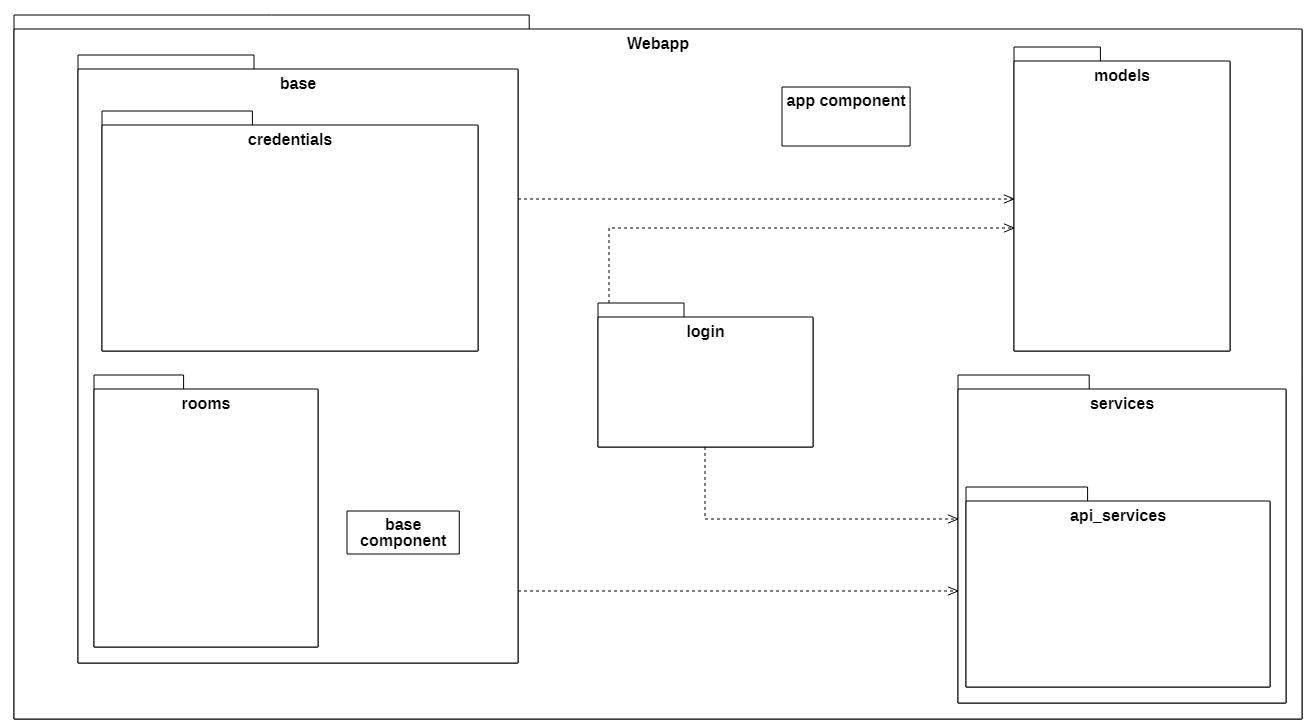
\includegraphics[width=18cm]{res/images/webapp-totale-diagrammaPackage.png}
	\caption{Diagramma dei package della webapp}
	\label{fig:DiagrammaPackageWebapp}
\end{figure}
Il diagramma sovrastante rappresenta la struttura e le relazioni dei package della webapp.

\subsubsection{Base}
\begin{figure}[H]
	\centering
	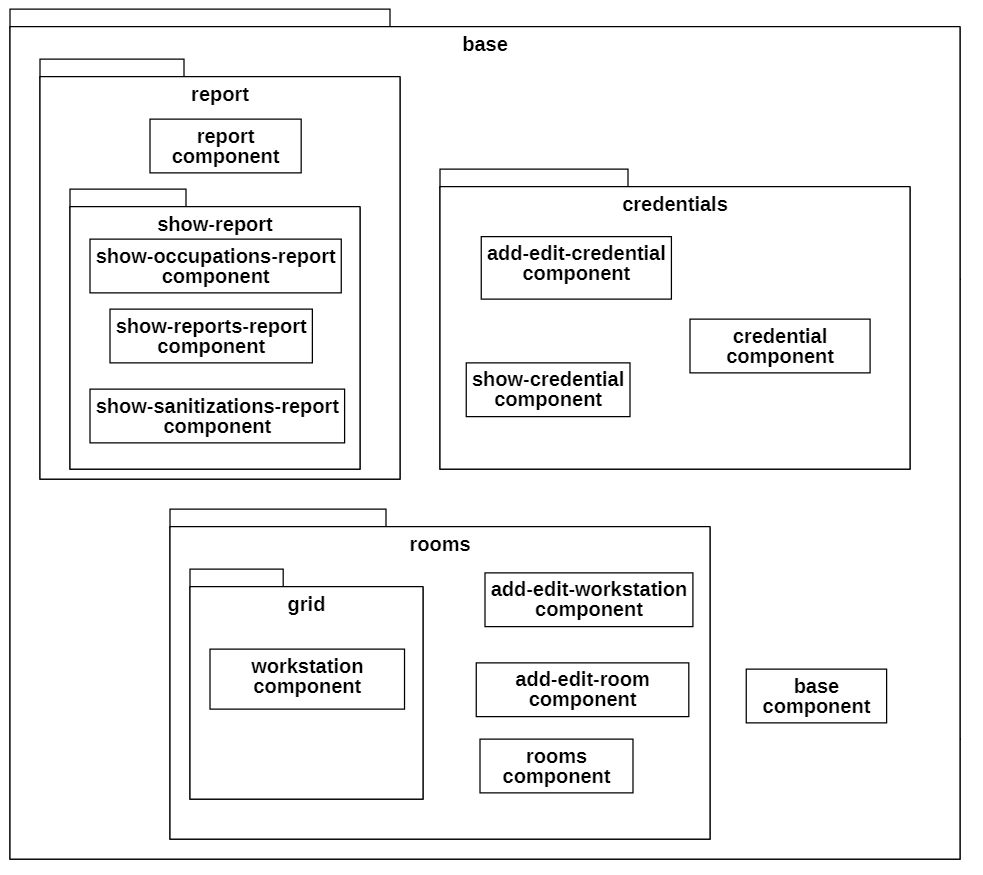
\includegraphics[width=13cm]{res/images/webapp-base-diagrammaPackage.png}
	\caption{Diagramma del package base della webapp}
	\label{fig:DiagrammaPackageBaseWebapp}
\end{figure}
Il package Base contiene tutte le funzionalità offerte a un amministratore autenticato.
Esse sono ulteriormente suddivise in due package:
\begin{itemize}
	\item Credentials
	\item Rooms
\end{itemize}
All'interno del package Credentials sono presenti tutti e soli i componenti utilizzati nella pagina di gestione delle credenziali. All'interno del package Rooms sono presenti tutti e soli i componenti utilizzati nella pagina di gestione delle stanze e delle postazioni. Le due pagine appena indicate sono annidate nella vista del componente Base. Quest'ultimo infatti presenta dei pulsanti per la selezione della pagina da visualizzare. Esso presenta inoltre, sempre tramite un pulsante, la funzionalità di logout. \newline
Il package Base ha una dipendenza verso Models, le cui classi vengono usate per organizzare i dati, e una verso Services, le cui classi vengono usate per interagire con il server e con il local storage.

\subsubsection{Login}
\begin{figure}[H]
	\centering
	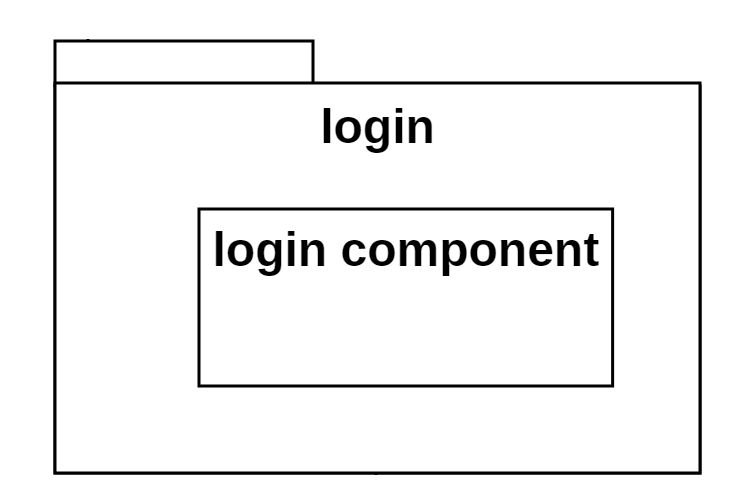
\includegraphics[width=5cm]{res/images/webapp-login-diagrammaPackage.png}
	\caption{Diagramma del package login della webapp}
	\label{fig:DiagrammaPackageLoginWebapp}
\end{figure}
Il package Login contiene le funzionalità necessarie per l'autenticazione dell'utente.

\subsubsection{Models}
\begin{figure}[H]
	\centering
	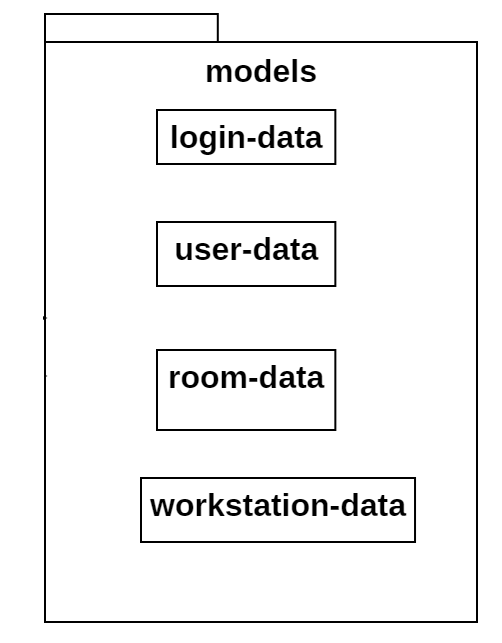
\includegraphics[width=10cm]{res/images/webapp-models-diagrammaPackage.png}
	\caption{Diagramma del package models della webapp}
	\label{fig:DiagrammaPackageModelsWebapp}
\end{figure}
Il package Models contiene le classi che vengono usate nel resto dell'applicazione per formattare i dati e comunicarli in modo ordinato e coeso.

\subsubsection{Services}
\begin{figure}[H]
	\centering
	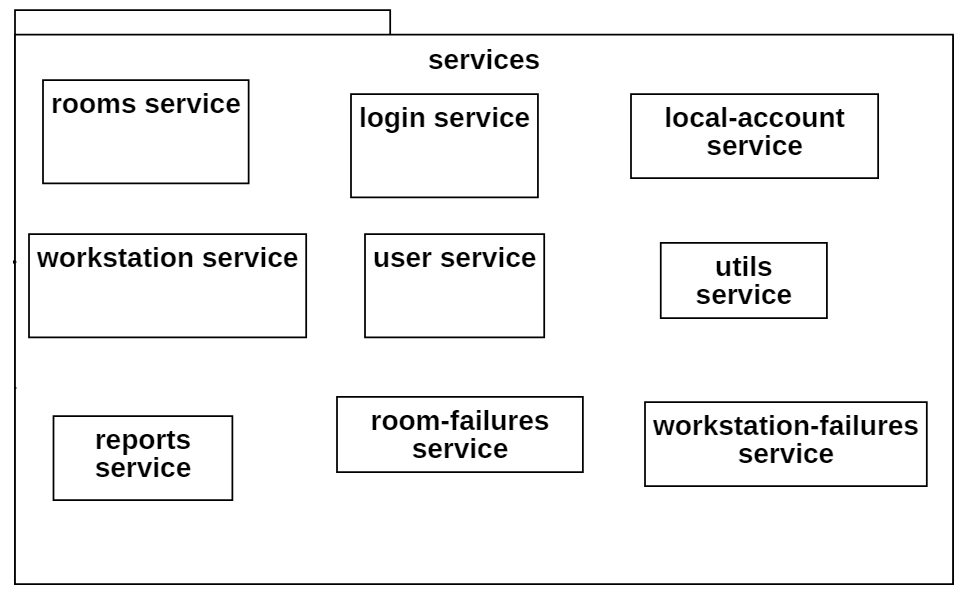
\includegraphics[width=12cm]{res/images/webapp-services-diagrammaPackage.png}
	\caption{Diagramma del package services della webapp}
	\label{fig:DiagrammaPackageServicesWebapp}
\end{figure}
Il package Services contiene le classi usate nel resto dell'applicazione per interagire col server e con il local storage oppure che fungono da contenitori di algoritmi comuni.

\subsection{Diagrammi delle classi}
Nei diagrammi e nelle descrizioni che seguono si possono notare alcune mancanze, di cui illustriamo ora le motivazioni:

\textbf{Diagrammi}
\begin{itemize}
	\item non sono rappresentate le classi HttpClient, Observable, UtilsService e le dipendenze verso di esse perchè sono molto comuni ed è quindi poco utile rappresentarle singolarmente. In particolare:
	\begin{itemize}
		\item \textbf{HttpClient}: classe fornita da Angular per eseguire chiamate http. Da questa classe dipendono tutti i servizi che si connettono al backend.
		\item \textbf{Observable}: classe fornita dalla libreria rxjs (Reactive Extensions) per ricezione di dati in modo asincrono. Ne sono dipendenti tutti servizi che si connettono al server e tutti i componenti che utilizzano quei servizi.
		\item \textbf{UtilsService}: servizio che offre alcuni algoritmi comuni. Ne dipendono quasi tutti i componenti e nessun servizio.
	\end{itemize}
\end{itemize}
\textbf{Descrizioni}
\begin{itemize}
	\item non sono presenti i costruttori delle classi perché essi non hanno alcun effetto oltre a quello di creare gli oggetti;
	\item per le classi del package Models non sono descritti gli attributi poiché essi sono semplicemente la copia delle informazioni contenute nel database;
	\item per le classi legate a un form accessibile all'utente non sono descritti gli attributi inseribili perché essi sono un sottoinsieme di quelli di cui si parla al punto precedente.
\end{itemize}

\subsubsection{Login}
\begin{figure}[H]
	\centering
	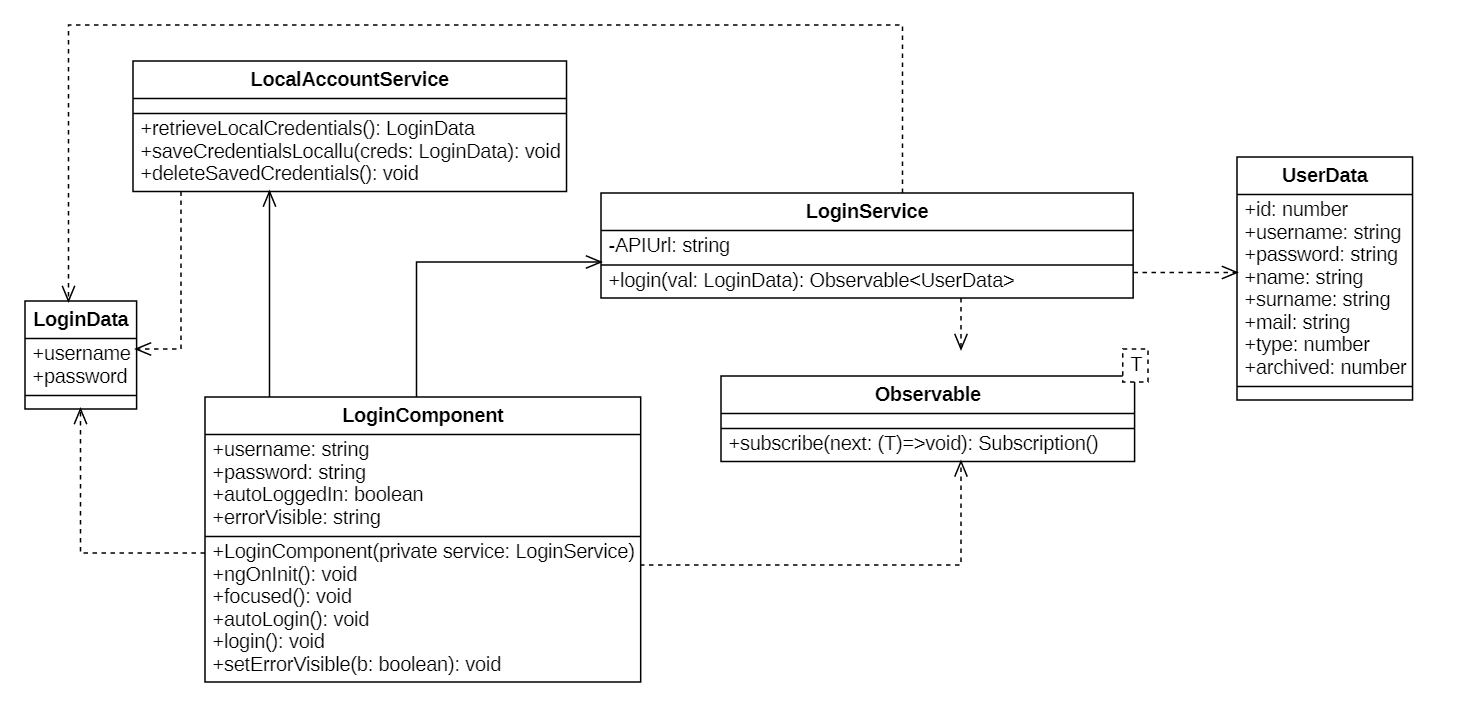
\includegraphics[width=18cm]{res/images/webapp-login-diagrammaClassi.png}
	\caption{Diagramma delle classi per il login}
	\label{fig:DiagrammaClassiLogin}
\end{figure}
Nel diagramma sovrastante sono rappresentate le classi utilizzate dalla pagina di login e le dipendenze tra di esse. La classe \texttt{LoginComponent} dirige la gestione del login manuale, tramite inserimento delle credenziali da parte dell'utente, e di quello automatico, tramite verifica delle credenziali precedentemente salvate nel local storage del browser. A \texttt{LoginService}, in particolare, viene delegata la verifica delle credenziali tramite il server, mentre a LocalAccountService, vengono delegate la scrittura, la lettura e l'eliminazione delle credenziali salvate nel browser. Per comunicare credenziali di accesso da una classe all'altra, viene utilizzata \texttt{LoginData}. \texttt{UserData} invece viene usata per la ricezione dal server dei dati dell'utente che si è autenticato.

\paragraph{Classi}

\subparagraph{LoginComponent}
Classe che si occupa della gestione del login manuale, ovvero tramite l'inserimento delle credenziali da parte dell'utente, e di quello automatico, ovvero tramite l'utilizzo delle credenziali precedentemente salvate nel local storage del browser. \newline
Questa classe contiene i seguenti attributi:
\begin{itemize}
	\item \textbf{autoLoggedIn: boolean} \newline
	Variabile utilizzata per memorizzare il successo o meno del login automatico.
	\item \textbf{errorVisible: string} \newline
	Variabile che determina la visibilità dell'errore mostrato all'utente.
\end{itemize}
Questa classe presenta i seguenti metodi:
\begin{itemize}
	\item \textbf{ngOnInit(): void} \newline
	Metodo che viene chiamato all'inizializzazione della pagina. Provoca l'evento di login automatico.
	\item \textbf{focused(): void} \newline
	Metodo che viene chiamato nel momento in cui uno dei due campi di inserimento delle credenziali viene selezionata. Provoca l'impostazione dell'invisibilità dell'errore che indica l'incorrettezza delle credenziali inserite.
	\item \textbf{autoLogin(): void} \newline
	Metodo che effettua un tentativo di autenticazione con le credenziali salvate nel local storage. Se l'autenticazione riesce l'utente viene reindirizzato alla pagina home. Altrimenti viene visualizzata la pagina di inserimento delle credenziali.
	\item \textbf{login(): void} \newline
	Metodo che effettua un tentativo di autenticazione con le credenziali inserite dall'utente. Se l'autenticazione riesce l'utente viene reindirizzato alla pagina home. Altrimenti viene mostrato un messaggio di errore.
	\item \textbf{setErrorVisible(b: boolean): void} \newline
	Metodo che imposta la visibilità dell'errore che indica l'incorrettezza delle credenziali inserite.
	\item \textbf{checkLoginResponse(data: UserData): void} \newline
	Metodo che indirizza l'utente alla pagina home se l'autenticazione ha avuto successo e mostra il form d login se l'autenticazione non ha avuto successo.
\end{itemize}
\subparagraph{LoginService}
Servizio che permette di verificare tramite il server la validità di credenziali per l'autenticazione. Ogni metodo di questa classe, tranne il costruttore, restituisce un \texttt{Observable}. Questo oggetto espone un metodo subscribe con il quale si potrà impostare una funzione di callback che verrà chiamata quando il server fornirà una risposta. \newline
Questa classe contiene i seguenti attributi:
\begin{itemize}
	\item \textbf{APIUrl: string}
	L'url base dell'API REST a cui il servizio fa riferimento.
\end{itemize}
Questa classe presenta i seguenti metodi:
\begin{itemize}
	\item \textbf{login(val: LoginData): Observable<UserData>} \newline
	Verifica l'esistenza delle credenziali passate come parametro nel database. Restituisce un Observable che permette di ottenere, in un \texttt{UserData}, i dati dell'utente corrispondente alle credenziali.
\end{itemize}
\subparagraph{LocalAccountService}
Servizio che permette di gestire il salvataggio delle credenziali dell'utente nel local storage del browser. \newline
Questa classe presenta i seguenti metodi:
\begin{itemize}
	\item \textbf{retrieveLocalCredentials(): LoginData} \newline
	Metodo che restituisce le credenziali salvate nel local storage. Se assenti restituisce un oggetto LoginData con i valori entrambi a null.
	\item \textbf{saveCredentialsLocally(creds: LoginData): void} \newline
	Metodo che salva le credenziali passate nel local storage.
	\item \textbf{deleteSavedCredentials(): void} \newline
	Metodo che elimina le credenziali salvate nel local storage.
	
\end{itemize}
\subparagraph{LoginData}
Classe che contiene i valori necessari per l'autenticazione di un amministratore al sistema. Viene usata per la comunicazione di questo tipo di dati all'interno dell'applicazione. \newline
\subparagraph{UserData}
Classe che contiene tutti e soli i valori necessari per il salvataggio di un utente sul database. È utilizzata per il transito dei dati degli utenti all'interno dell'applicazione. \newline

\subsubsection{Aggiunta e modifica stanze}
\begin{figure}[H]
	\centering
	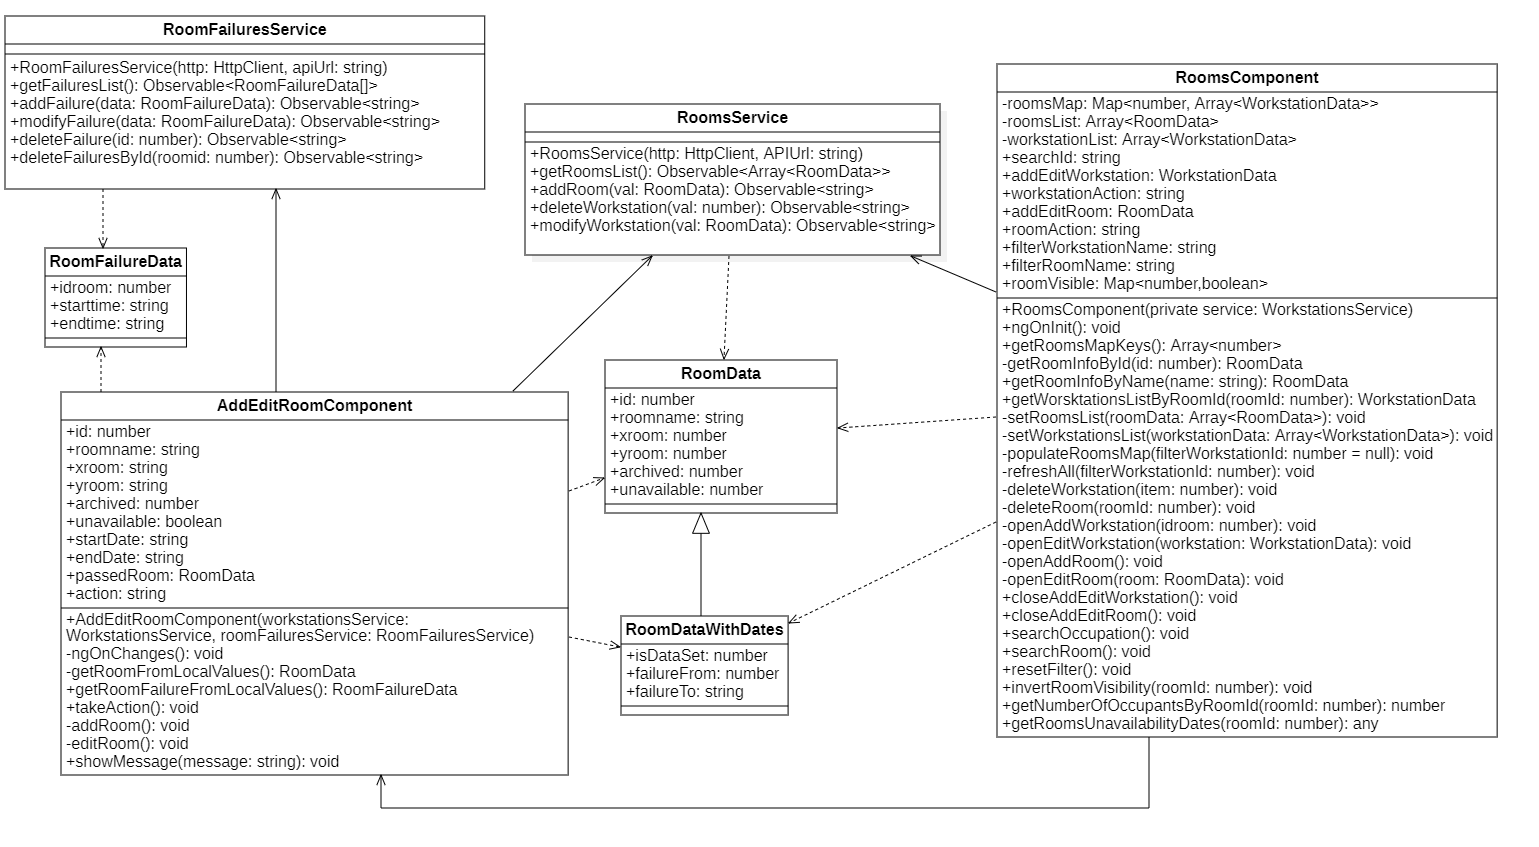
\includegraphics[width=18cm]{res/images/webapp-AddEditStanze-diagrammaClassi.png}
	\caption{Diagramma delle classi per la gestione delle stanze e delle postazioni}
	\label{fig:DiagrammaClassiStanzePostazioni}
\end{figure}
Il diagramma sovrastante rappresenta l'architettura utilizzata per l'aggiunta e modifica delle stanze. \newline
\texttt{RoomsComponent} si occupa della visualizzazione ed eliminazione delle stanze. Essa delega la creazione e modifica di questi due dati alla classe \texttt{AddEditRoomComponent}. Le due componenti contengono riferimenti ai servizi di cui necessitano. I due servizi coinvolti sono \texttt{RoomService} e \texttt{RoomFailuresService}. Le informazini vengono ottenute dal server tramite la classe \texttt{Observable}. In generale i dati riguardanti le stanze sono scambiati utilizzando le due classi \texttt{RoomData} e \texttt{RoomDataWithDates}.

L'aggiunta e modifica delle postazioni è molto simile al caso qui presentato. Pertanto esse non vengono illustrate.


\paragraph{Classi}
\subparagraph{RoomsComponent}
Classe che si occupa della visualizzazione, eliminazione e, tramite i componenti AddEditWorkstation e AddEditRoom, dell'aggiunta e modifica di postazioni e stanze. \newline
Questa classe contiene i seguenti attributi:
\begin{itemize}
	\item \textbf{roomsMap: Map<number, Array<WorkstationData> >} \newline
		Map in cui ad ogni stanza sono assegnate le sue postazioni, ovvero quelle con \texttt{idroom} uguale all'\texttt{id} della stanza. Se l'utente applica un filtro alla lista, qui verranno contenute solo le stanze e le postazioni selezionate da tale filtro.
	\item \textbf{roomsList: Array<RoomsData>} \newline
		Array utilizzato per contenere le stanze ottenute dal server.
	\item \textbf{workstationList: Array<Workstation>} \newline
		Array utilizzato per contenere le postazioni ottenute dal server.
	\item \textbf{searchId: string} \newline
		Id specificato dall'utente per la ricerca di una postazione.
	\item \textbf{addEditWorkstation: WorkstationData} \newline
		Contiene i dati della postazione che verrà aggiunta o modificata.
	\item \textbf{workstationAction: string} \newline
		Valore specificato dall'utente che provocherà la modifica o l'aggiunta della postazione salvata in \texttt{addEditWorkstation}.
	\item \textbf{addEditRoom: RoomData} \newline
		Contiene i dati della stanza che verrà aggiunta o modificata.
	\item \textbf{roomAction: string} \newline
		Valore specificato dall'utente che provocherà la modifica o l'aggiunta della stanza salvata in \texttt{addEditRoom}.
\end{itemize}
Questa classe presenta i seguenti metodi:
\begin{itemize}
	\item \textbf{ngOnInit(): void} \newline
	Questa funzione viene chiamata all'inizializzazione della pagina e provoca l'aggiornamento di roomsMap.
	\item \textbf{getRoomsMapKeys(): Array<number>} \newline
	Restituisce un array con gli id delle stanze contenute in \texttt{roomsMap}.
	\item \textbf{getRoomInfoById(id: number): RoomData} \newline
	Restituisce un oggetto \texttt{RoomData} con i dati della stanza identificata dall'id passato come parametro.
	\item \textbf{setRoomList(roomData: Array<RoomData>): void} \newline
	Reinizializza \texttt{roomList} con i dati ricevuti
	\item \textbf{setWorkstationList(workstationData: Array<WorkstationData>): void} \newline
	Reinizializza \texttt{workstationList} con i dati ricevuti
	\item \textbf{populateRoomsMap(filterWorkstationId: number): void} \newline
	Reinizializza \texttt{roomsMap} ponendo come chiavi gli id delle stanze contenute in \texttt{roomsList} e come valori le postazioni contenute nelle rispettive stanze. In questo modo sarò facile ottenere le postazioni contenute in una stanza conoscendo l'id di quest'ultima. \newline
	Se non viene specificato l'attributo \texttt{filterWorkstationId} nella mappa vengono inserite anche le stanze vuote. \newline
	Se viene specificato l'attributo \texttt{filterWorkstationId} verrà inserita nella mappa solo la postazione con l'id indicato e la stanza che la contiene.
	\item \textbf{refreshAll(filterWorkstationId: number): void} \newline
	Richiede al server le stanze e le postazioni e le organizza, tramite \texttt{populateRoomsMap}, in una mappa. Il parametro \texttt{filterWorkstationId} viene passato direttamente a \texttt{populateRoomsMap}
	\item \textbf{deleteWorkstation(item: number): void} \newline
	Richiede al server l'eliminazione della postazione con l'id specificato
	\item \textbf{deleteRoom(roomId: number): void} \newline
	Richiede al server l'eliminazione della stanza con l'id specificato
	\item \textbf{openAddWorkstation(idroom: number): void} \newline
	Rende visibile il form per l'aggiunta di una postazione. Inoltre imposta i parametri necessari all'esecuzione di questa azione.
	\item \textbf{openEditWorkstation(workstation: WorkstationData): void} \newline
	Rende visibile il form per la modifica di una postazione. Inoltre imposta i parametri necessari all'esecuzione di questa azione. 
	\item \textbf{openAddRoom(): void} \newline
	Rende visibile il form per l'aggiunta di una stanza. Inoltre imposta i parametri necessari all'esecuzione di questa azione.
	\item \textbf{openEditRoom(room: RoomData): void} \newline
	Rende visibile il form per la modifica di una stanza. Inoltre imposta i parametri necessari all'esecuzione di questa azione.
	\item \textbf{closeAddEditWorkstation(): void} \newline
	Provoca l'aggiornamento dei dati contenuti nella pagina.
	\item \textbf{closeAddEditRoom(): void} \newline
	Provoca l'aggiornamento dei dati contenuti nella pagina.
	\item \textbf{searchWorkstation(): void} \newline
	Richiede tutti i dati sulle postazioni e sulle stanze al server specificando il filtro indicato dall'utente.
	\item \textbf{resetFilter(): void} \newline
	Richiede tutti i dati sulle postazioni e sulle stanze al server senza alcun filtro.
\end{itemize}
	

\subparagraph{AddEditRoomComponent}
Classe che si occupa dell'aggiunta e modifica di stanze. I primi 5 attributi sono sempre sincronizzati con il form che viene presentato all'utente. Tramite essi viene definita la stanza da aggiungere o i nuovi dati della stanza da modificare.\newline
Questa classe contiene i seguenti attributi:
\begin{itemize}
	\item \textbf{passedRoom: RoomData 	} \newline
	L'oggetto che viene passato da \texttt{RoomComponent} e che indica la stanza da modificare.
	\item \textbf{action: string} \newline
	L'attributo che viene passato da \texttt{RoomComponent} e che indica il tipo di azione da eseguire: aggiunta o modifica della stanza;
\end{itemize}
Questa classe presenta i seguenti metodi:
\begin{itemize}
	\item \textbf{ngOnChanges(): void 	} \newline
	Metodo chiamato ogni volta che una proprietà data-bound viene modificata. In questo caso serve per aggiornare i parametri locali in base ai valori di \texttt{passedRoom}.
	\item \textbf{getRoomFromLocalValues(): RoomData 	} \newline
	Restituisce un oggetto \texttt{RoomData} ottenuto dai primi 5 attributi.
	\item \textbf{takeAction(): void 	} \newline
	Chiama il metodo \texttt{addRoom()} o \texttt{editRoom()} a seconda del valore dell'attributo action.
	\item \textbf{addRoom(): void 	} \newline
	Richiede al service di aggiungere la stanza specificata.
	\item \textbf{editRoom(): void} \newline
	Richiede al service di modificare la postazione nel modo specificato.
	\item \textbf{showMessage(message: string): void} \newline
	Metodo che mostra all'utente la stringa passata come parametro.
\end{itemize}

\subparagraph{RoomsService}
Servizio che permette di ottenere dal server informazioni sulle stanze. Ogni metodo di questa classe, tranne il costruttore, restituisce un \texttt{Observable}. Questo oggetto espone un metodo subscribe con il quale si potrà impostare una funzione di callback che verrà chiamata quando il server fornirà una risposta. \newline
Questa classe contiene i seguenti attributi:
\begin{itemize}
	\item \textbf{APIUrl: string} \newline
	L'url base dell'API REST a cui il servizio fa riferimento.
\end{itemize}
Questa classe presenta i seguenti metodi:
\begin{itemize}
	\item \textbf{getRoomsList(): Observable<Array<RoomData> > 	} \newline
	Usato per ottenere una lista delle stanze.
	\item \textbf{addRoom(val: RoomData): Observable<string> 	} \newline
	Usato per tentare di aggiungere la stanza indicata in \texttt{val} e di ricevere l'esito dell'operazione.
	\item \textbf{deleteWorkstation(val: number): Observable<string> 	} \newline
	Usato per tentare di eliminare la stanza con id \texttt{val} e di ricevere l'esito dell'operazione.
	\item \textbf{modifyWorkstation(val: RoomData): Observable<string>} \newline
	Usato per tentare di modificare la stanza con id pari a quello contenuto in \texttt{val} assegnandole gli altri valori dello stesso parametro. Restituisce, tramite un \texttt{Observable}, una risposta in formato stringa che indica l'esito dell'operazione.
\end{itemize}
\subparagraph{RoomData}
Questa classe contiene tutti e soli i valori necessari per il salvataggio di una stanza sul database. È utilizzata per il transito dei dati delle stanze all'interno dell'applicazione. \newline

\subsubsection{Visualizzazione stanze e postazioni}
\begin{figure}[H]
	\centering
	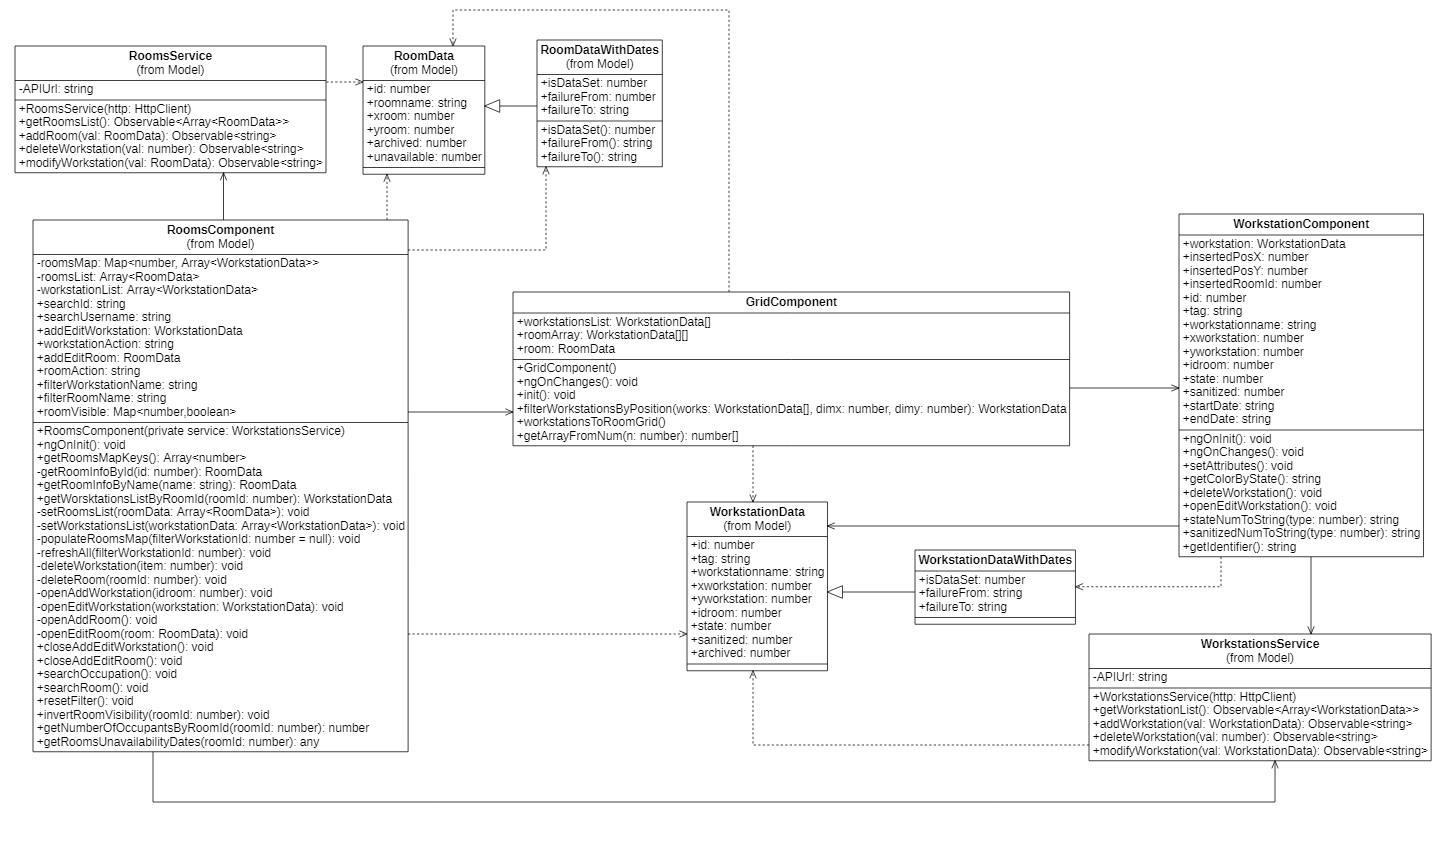
\includegraphics[width=18cm]{res/images/webapp-visualStanzePostazioni-diagrammaClassi.png}
	\caption{Diagramma delle classi per la visualizzazione delle stanze e delle postazioni}
	\label{fig:DiagrammaClassiVisualStanzePostazioni}
\end{figure}

\paragraph{Classi}
Alla visualizzazione delle stanze e delle postazioni prendono parte le componenti \texttt{RoomsComponent}, \texttt{GridComponent}, \texttt{WorkstationComponent} che gestiscono i dati a tre livelli diversi, dal più alto al più basso.
I dati vengono gestiti e trasportati tramite le classi \texttt{RoomData}, \texttt{RoomDataWithDates}, \texttt{WorkstationData}, \texttt{WorkstationDataWithDates}.
I dati vengono ottenuti dal server tramite i due servizi \texttt{RoomsService} e \texttt{WorkstationsService}.

Di seguito viene descritto meglio il ruolo delle classi. Vengono esclusi i metodi non strettamente inerenti alla visualizzazione delle stanze e delle postazioni e i metodi il cui funzionamento è facilmente deducibile dal nome.
\subparagraph{RoomsComponent}
Si occupa di ottenere le stanze e le postazioni dal server, tramite il metodo \texttt{refreshAll} e di organizzare le seconde all'interno delle prime tramite il metodo \texttt{populateRoomsMap}. Il primo metodo scarica in modo parallelo i dati dal server e li salva negli array \texttt{roomsList} e \texttt{workstationList}. Il secondo metodo invece prende le postazioni appena raccolte e le suddivide per stanza nella mappa <number, WorsktationData> \texttt{roomsMap}.
Una volta popolate le stanze, è possibile assegnare ad ogni \texttt{GridComponent} le postazioni corrispondenti.
\subparagraph{GridComponent}
Si occupa di organizzare le postazioni ricevute in una matrice e di visualizzare quest'ultima in un tabella html. Le postazioni sono salvate nell'array \texttt{workstationsList} mentre la matrice è \texttt{roomArray}. L'organizzazione viene eseguita tramite il metodo \texttt{workstationsToRoomGrid}. Una volta eseguita viene assegnata ad ogni WorkstationComponent la rispettiva postazione.
\subparagraph{WorkstationComponent}
Questo componente si occupa di rappresentare la postazione ricevuta. Questa rappresentazione avviene esponendo nella vista (html) gli attributi della postazione e colorando il componente con un colore consono allo stato e alla situazione di sanificazione. Questo colore viene calcolato tramite il metodo \texttt{getColorByState}.
\subparagraph{Classi Data}
Come suggerito dai nomi, i dati sono rappresentati in due formati: con e senza date.
Questa variabilità dipende dallo stato di inaccessibilità della stanza o della postazione. Nel caso in cui essa sia inaccessibile, sono indicate anche le date di inizio e fine del perido in cui tale stato sarà vigente.
\subparagraph{Servizi}
I due servizi utilizzati forniscono entrambi 4 metodi in formato CRUD (Create, Read, Update, Delete) che rispecchiano le API fornite dal backend.


\subsubsection{Gestione credenziali}
\begin{figure}[H]
	\centering
	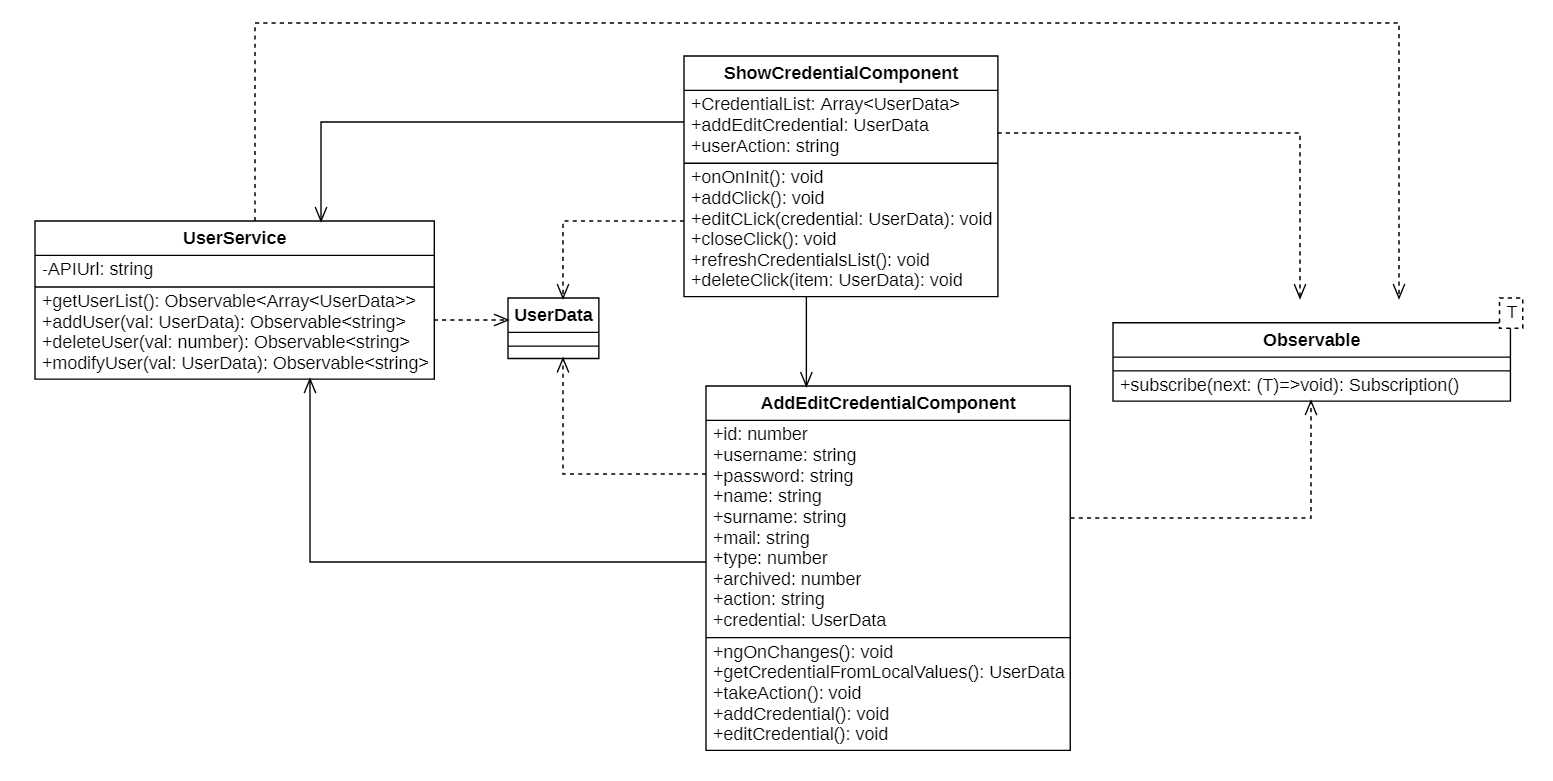
\includegraphics[width=18cm]{res/images/webapp-credenziali-diagrammaClassi.png}
	\caption{Diagramma delle classi per la gestione delle credenziali}
	\label{fig:DiagrammaClassiCredenziali}
\end{figure}
Il diagramma delle classi sovrastante rappresenta le classi coinvolte nella pagina di gestione delle credenziali e le loro relazioni. Il funzionamento di questa pagina è simile a quello della pagina di gestione delle stanze e delle postazioni. Qui la classe \texttt{ShowCredentialComponent} si occupa di ottenere la lista delle credenziali dal servizio \texttt{UserService} tramite oggetti \texttt{Observable}. Essa delega alla classe \texttt{AddEditCredentialComponent} l'aggiunta e modifica di credenziali. Il passaggio delle informazioni riguardanti le credenziali viene sempre attuato tramite oggetti della classe \texttt{UserData}.

\paragraph{Classi}
\subparagraph{ShowCredentialComponent}
Classe che si occupa della visualizzazione di una lista delle credenziali ottenute tramite il service \texttt{UserService}. \newline
Questa classe contiene i seguenti attributi:
\begin{itemize}
	\item \textbf{CredentialList: Array<UserData>} \newline
	Array nel quale vengono salvate le credenziali ottenute dal service.
	\item \textbf{addEditCredential: UserData} \newline
	Variabile utilizzata per il passaggio delle informazione da questa classe a \texttt{AddEditCredentialComponent}. Il valore di questa variabile viene assegnato alla variabile \texttt{credential} di quest'ultima classe.
	\item \textbf{userAction: string} \newline
	Variabile utilizzata per la selezione del tipo di azione (aggiunta o modifica) da eseguire. Il valore di questa variabile viene assegnato alla variabile \texttt{action} di \texttt{AddEditCredentialComponent}.
\end{itemize}
Questa classe presenta i seguenti metodi:
\begin{itemize}
	\item \textbf{ngOnInit(): void} \newline
	Metodo chiamato all'inizializzazione della pagina. Provoca l'aggiornamento della lista di credenziali.
	\item \textbf{addClick(): void} \newline
	Metodo chiamato nel momento in cui l'utente apre il form di creazione di una credenziale. Imposta \texttt{userAction} e \texttt{addEditCredential} in modo che possano essere usate per aggiungere una credenziale al sistema.
	\item \textbf{editClick(credential: UserData): void} \newline
	Metodo chiamato nel momento in cui l'utente apre il form di modifica di una credenziale. Imposta \texttt{userAction} e \texttt{addEditCredential} in modo che possano essere usate per modificare la credenziale.
	\item \textbf{closeClick(): void} \newline
	Metodo chiamato nel momento in cui l'utente chiude il form di creazione di una credenziale. Provoca l'aggiornamento della lista di credenziali.
	\item \textbf{refreshCredentialsList(): void} \newline
	Provoca l'aggiornamento della lista di credenziali tramite \texttt{UserService}.
	\item \textbf{deleteClick(item: UserData): void} \newline
	Metodo chiamato nel momento in cui l'utente preme sul pulsante per l'eliminazione di una credenziale. Provoca l'eliminazione tramite \texttt{UserService}.
\end{itemize}
\subparagraph{AddEditCredentialComponent}
Classe che si occupa della creazione e modifica di credenziali da parte dell'utente. I primi 8 attributi sono modificabili dall'utente tramite un form e definiscono i valori della credenziale che si sta creando o modificando. \newline
Questa classe contiene i seguenti attributi:
\begin{itemize}
	\item \textbf{action: string} \newline
	Variabile che determina il tipo di azione da eseguire ( aggiunta o modifica della credenziale). Viene impostata dalla classe \texttt{ShowCredentialComponent}.
	\item \textbf{credential: UserData} \newline
	Variabile attraverso la quale questa classe ottiene i valori iniziali della credenziale che dovrà essere modificata o aggiunta. Viene impostata dalla classe \texttt{ShowCredentialComponent}.
\end{itemize}
Questa classe presenta i seguenti metodi:
\begin{itemize}
	\item \textbf{ngOnChanges(): void} \newline
	Metodo chiamato ogni volta che uno degli attributi data-bound, in questo caso \texttt{action} e \texttt{credential} viene modificato. Viene utilizzato per aggiornare i primi 8 attributi in base al valore dell'ultimo, che viene impostato da \texttt{ShowCredentialComponent}.
	\item \textbf{getCredentialFromLocalValues(): UserData} \newline
	Restituisce un oggetto costruito a partire dai primi 8 attributi della classe.
	\item \textbf{takeAction(): void} \newline
	Avvia l'evento di aggiunta o modifica della credenziale. La scelta tra le due possibilità è determinata dall'attributo action.
	\item \textbf{addCredential(): void} \newline
	Aggiunge la credenziale determinata dai primi 8 valori al server.
	\item \textbf{editCredential(): void} \newline
	Modifica la credenziale presente sul server con id pari all'attributo \texttt{id} impostandone gli altri valori con quelli degli altri attributi.
	\item \textbf{showMessage(message: string): void} \newline
	Metodo che mostra all'utente la stringa passata come parametro.
\end{itemize}
\subparagraph{UserService}
Servizio che permette di ottenere dal server le credenziali salvate. Ogni metodo di questa classe, tranne il costruttore, restituisce un \texttt{Observable}. Questo oggetto espone un metodo subscribe con il quale si potrà impostare una funzione di callback che verrà chiamata quando il server fornirà una risposta. \newline
Questa classe contiene i seguenti attributi:
\begin{itemize}
	\item \textbf{APIUrl: string}
	L'url base dell'API REST a cui il servizio fa riferimento.
\end{itemize}
Questa classe presenta i seguenti metodi:
\begin{itemize}
	\item \textbf{getUserList(): Observable<Array<UserData> >} \newline
	Fornisce un'array contenente tutte le credenziali presenti sul server
	\item \textbf{addUser(val: UserData): Observable<string>} \newline
	Permette di aggiungere una credenziale al server. Restituisce l'esito dell'operazione sotto forma di stringa.
	\item \textbf{deleteUser(val: number): Observable<string>} \newline
	Permette di rimuovere una credenziale dal server, specificandone l'id. Restituisce l'esito dell'operazione sotto forma di stringa.
	\item \textbf{modifyUser(val: UserData): Observable<string>} \newline
	Permette di modificare una credenziale presente sul server. La credenziale da modificare è specificata dall'attributo \texttt{id} del parametro \texttt{val}. I nuovi valori della credenziale sono specificati dagli altri attributi del parametro. Restituisce l'esito dell'operazione sotto forma di stringa.
\end{itemize}
\subparagraph{UserData}
Questa classe contiene tutti e soli i valori necessari per il salvataggio di un utente sul database. È utilizzata per il transito dei dati degli utenti all'interno dell'applicazione. \newline

\subsubsection{Visualizzazione report}
\begin{figure}[H]
	\centering
	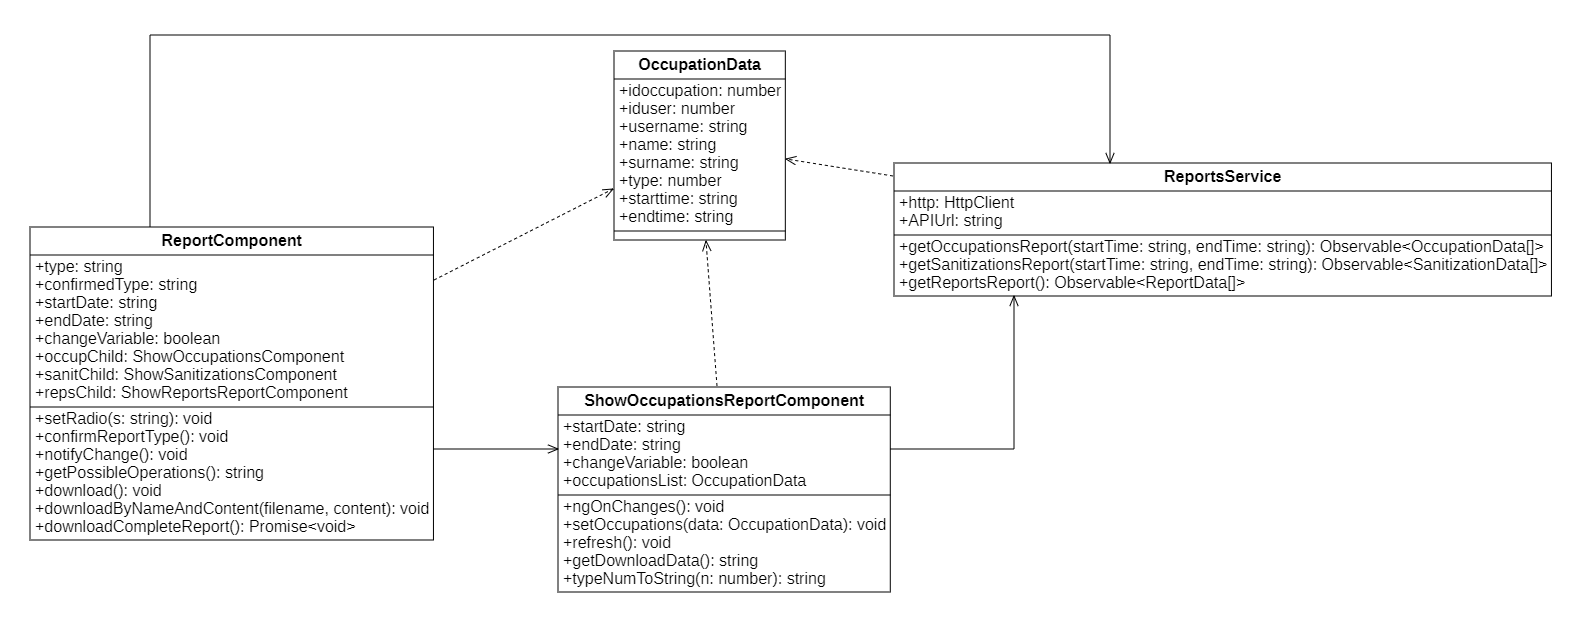
\includegraphics[width=18cm]{res/images/webapp-report-diagrammaClassi.png}
	\caption{Diagramma delle classi per la visualizzazione dei report}
	\label{fig:DiagrammaClassiReport}
\end{figure}

\paragraph{Classi}
Le classi prese in considerazione nel diagramma servono per la visualizzazione del report delle occupazioni.
\subparagraph{ReportComponent}
Fornisce un'interfaccia per:
\begin{itemize}
	\item selezione tipo di report da visaulizzazione o scaricare;
	\item filtraggio report per periodo;
	\item scaricamento report.
\end{itemize}
\subparagraph{ShowOccupationsReportComponent}
Questo componente si occupa di ottenere una lista delle occupazioni tramite il metodo \texttt{refresh} e di mostrarle tramite la vista. Le occupazioni vengono filtrate in base al periodo definito dai valori di \texttt{startDate} e \texttt{endDate}. Inoltre questo componente fornisce, tramite il metodo \texttt{getDownloadData}, la lista delle occupazioni in formato csv. In questo modo \texttt{ReportComponent} può ottenere i dati da far scaricare all'utente.
\subparagraph{OccupationData}
Rappresenta una occupazione singola.
\subparagraph{ReportsService}
Fornisce tre metodi per ottenere i tre tipi di report possibili. I primi due metodi accettano in input due date che definiscono il periodo all'interno del quale si cercano le informazioni.

L'utilizzo dei componenti \texttt{ShowSanitizationsReportComponent} e \texttt{ShowReportsReportComponent} è quasi identico a quanto appena descritto. Pertanto esso non viene illustrato esplicitamente

\subsection{Diagrammi di sequenza}
\subsubsection{Login}
\begin{figure}[H]
	\centering
	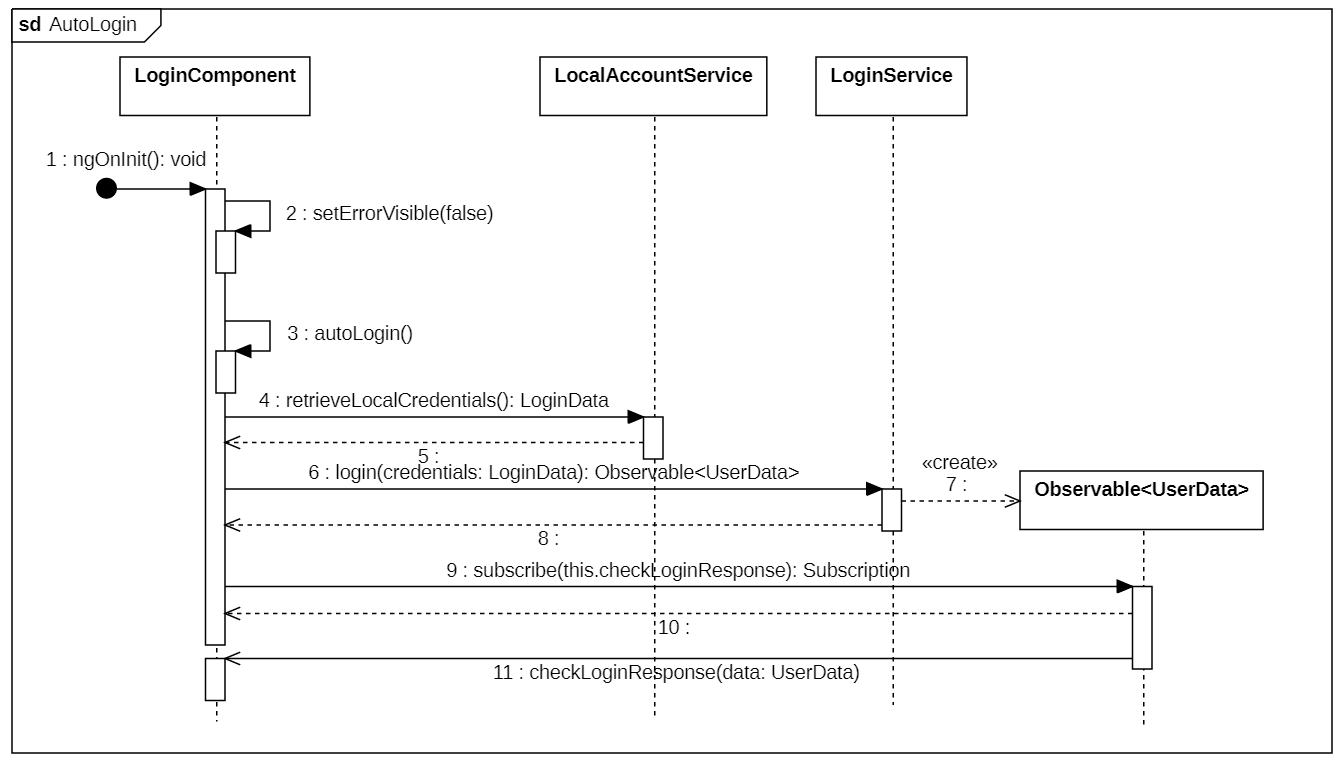
\includegraphics[width=18cm]{res/images/webapp-autologin-diagrammaSequenza.png}
	\caption{Diagramma di sequenza per l'evento di login automatico}
	\label{fig:DiagrammaSequenzaAutoLogin}
\end{figure}
Il diagramma sovrastante rappresenta l'evento di login automatico. L'evento è provocato dall'inizializzazione della pagina (\texttt{ngOnInit}). La sequenza consiste nel richiedere le credenziali salvate nel browser tramite il \texttt{LocalAccountService} ( \texttt{retrieveLocalCredentials}) e nel tentare un'autenticazione al server con esse tramite il metodo \texttt{login} del \texttt{LoginService}. In caso di esito positivo viene resituito da quest'ultimo servizio un oggetto \texttt{UserData} con i dati dell'utente che si è autenticato. La funzione \texttt{checkLoginResponse} gestisce la risposta del server provocando il reindirizzamento alla home page, in caso di successo, o la visualizzazione del form per l'inserimento delle credenziali.
\subsubsection{Gestione stanze e postazioni}
\begin{figure}[H]
	\centering
	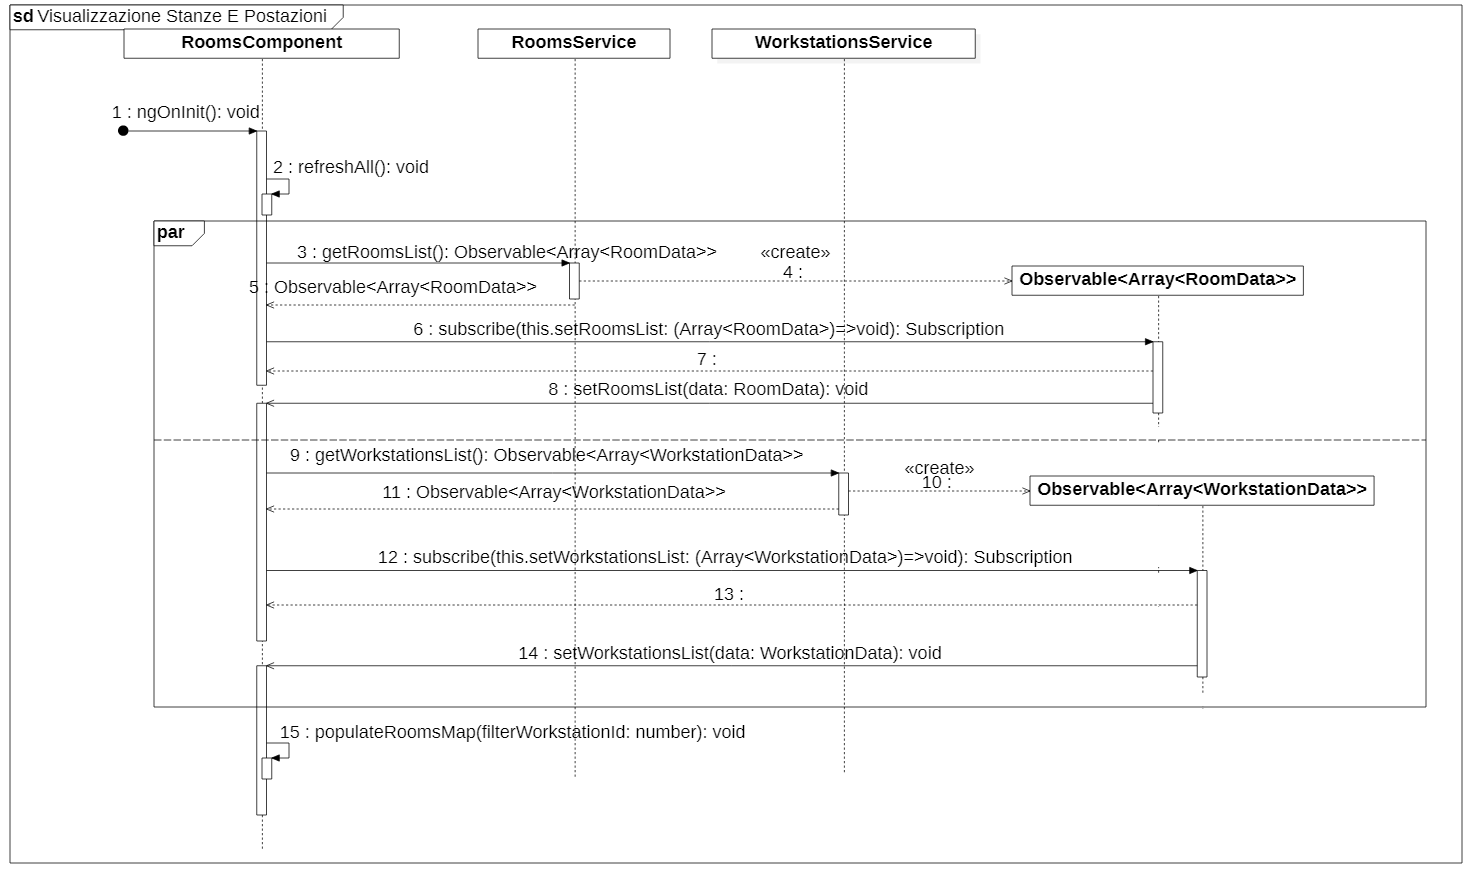
\includegraphics[width=18cm]{res/images/webapp-visualStanzePostazioni-diagrammaSequenza.png}
	\caption{Diagramma di sequenza per la visualizzazione delle stanze e delle postazioni}
	\label{fig:DiagrammaSequenzaStanzePostazioni1}
\end{figure}
L'evento rappresentato nel diagramma sovrastante è scatenato dalla chiamata di \texttt{ngOnInit}. Come conseguenza viene chiamato il metodo \texttt{refreshAll} che fa eseguire parallelamente due richieste di dati al server, la prima per ottenere le stanze e la seconda per ottenere le postazioni. In entrambe le esecuzioni il componente chiama il metodo apposito del servizio e riceve come risposta un \texttt{Observable}. Poi, chiamando il metodo \texttt{subscribe} di questo oggetto, il componente invia la chiamata al server e imposta la funzione di callback che ne gestirà la risposta. In entrambi i casi i dati di ritorno vengono assegnati a degli attributi del componente. Per le stanze il metodo \texttt{setRoomsList} assegna l'array di ritorno all'array locale \texttt{roomsList}. Per le stanze, invece, il metodo \texttt{setWorkstationsList} assegna l'array di ritorno all'array locale \texttt{workstationList}. Quando entrambe le risposte sono arrivate l'esecuzione procede col metodo \texttt{populateRoomsMap}, che organizza le stanze e le postazioni in una mappa.
Dal diagramma sono esclusi gli eventi successivi al popolamento delle stanze. In sostanza ai diversi GridComponent, rappresentanti le singole stanze, vengono assegnate le rispettive postazioni. All'interno del componente questi oggetti verrano ulteriormente organizzati in una matrice rappresentante la griglia. Per ogni elemento della matrice viene successivamente creato un WorkstationComponent e gli viene assegnata la rispettiva postazione, se presente.

\begin{figure}[H]
	\centering
	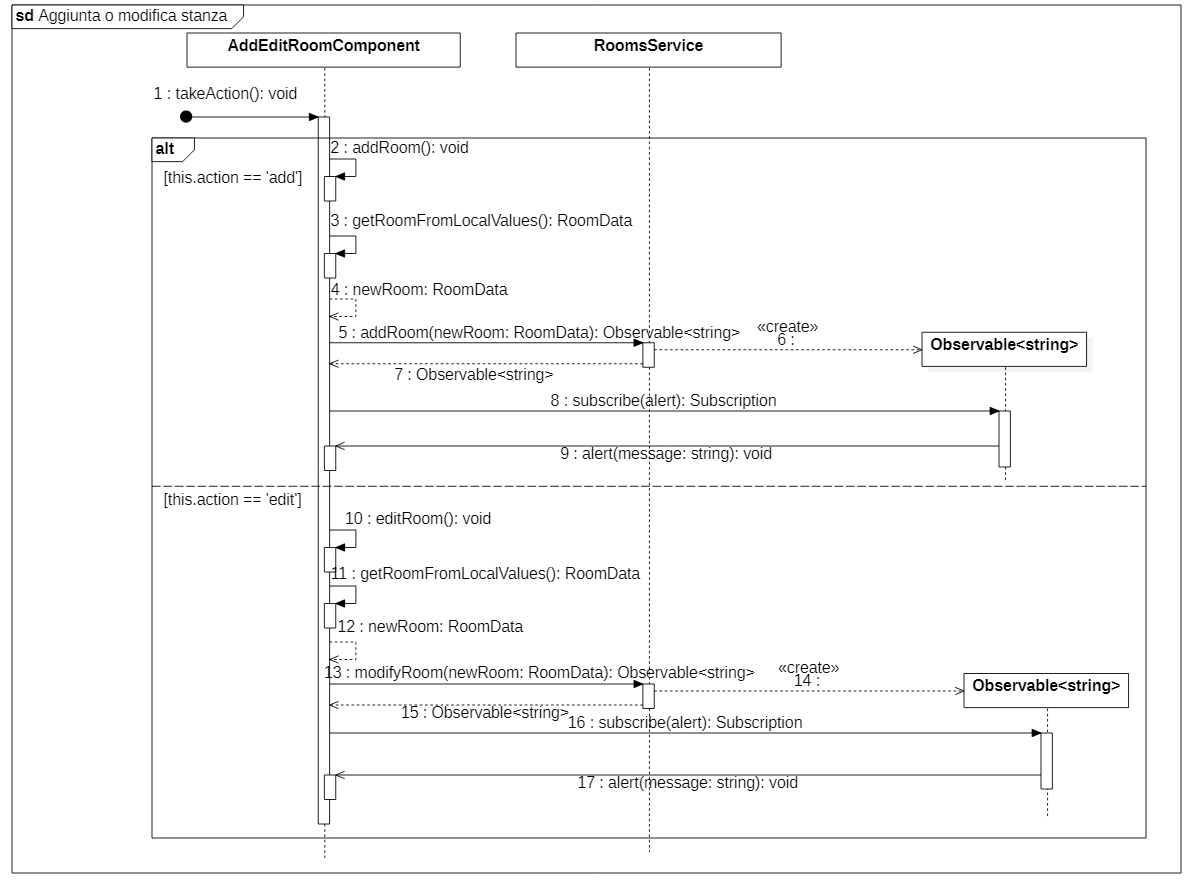
\includegraphics[width=18cm]{res/images/webapp-addEditStanzePostazioni-diagrammaSequenza.png}
	\caption{Diagramma di sequenza per l'aggiunta e la modifica di una stanza}
	\label{fig:DiagrammaSequenzaStanzePostazioni2}
\end{figure}

Il diagramma sovrastante rappresenta l'evento di aggiunta o modifica di una stanza.
L'azione è provocata dalla chiamata del metodo \texttt{takeAction} successiva alla pressione di un pulsante da parte dell'utente. A questo punto la scelta dell'una o dell'altra via è determinata dal parametro \texttt{action}, che ha assunto valore 'add' o 'edit' a seconda del pulsante premuto. In entrambi i casi l'azione è eseguita inviando i dati da inserire, formattati in un \texttt{RoomData}, al servizio. Il servizio restituisce un \texttt{Observable} che permette, tramite il metodo \texttt{subscribe}, di eseguire la chiamata al server e di impostare una funzione di callback per gestire i dati di ritorno. 
\subsubsection{Gestione credenziali}
\begin{figure}[H]
	\centering
	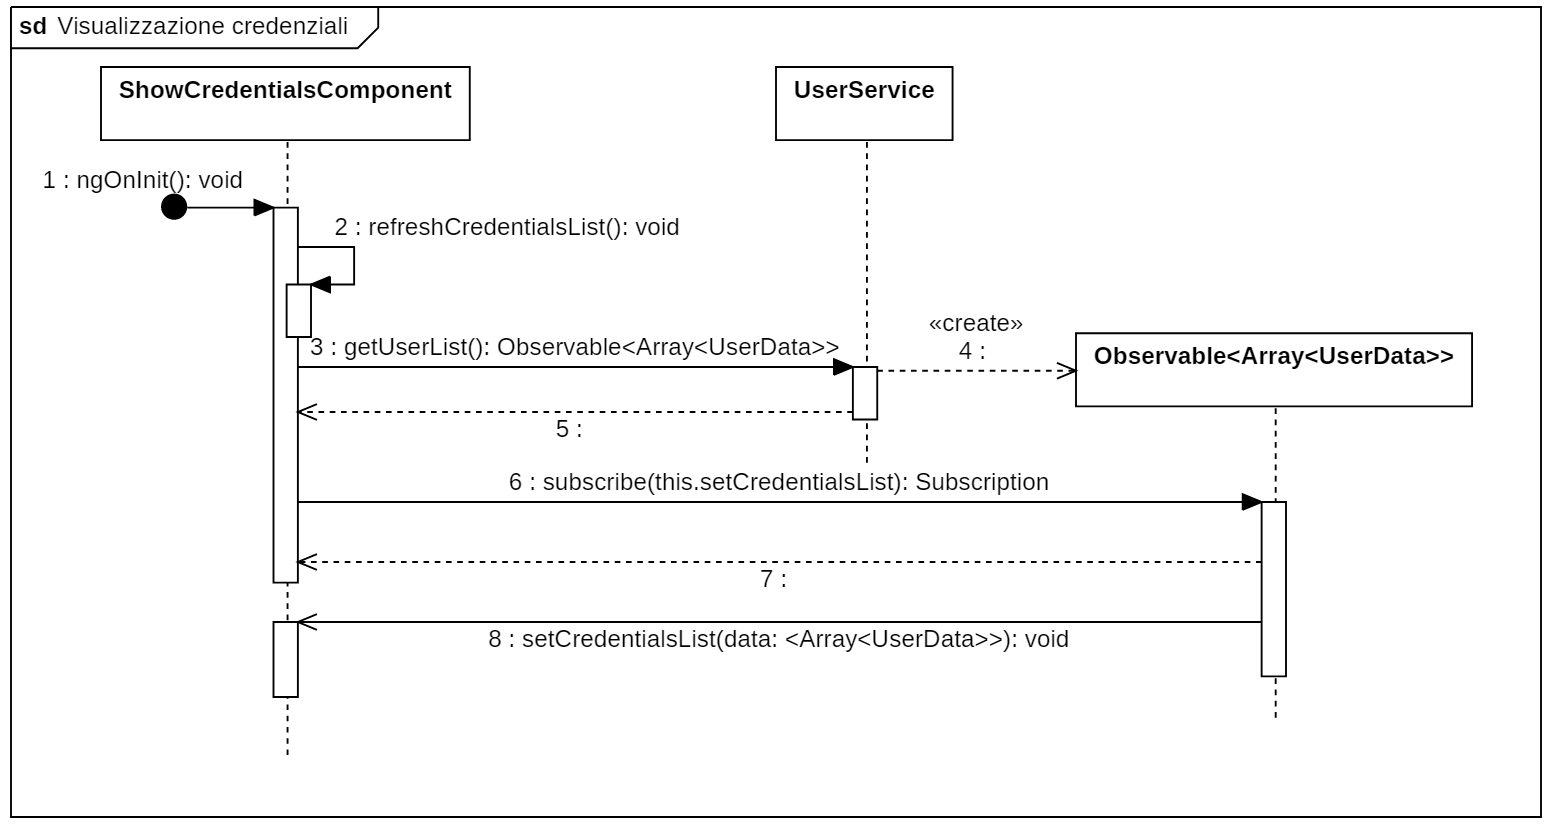
\includegraphics[width=18cm]{res/images/webapp-showCredentials-diagrammaSequenza.png}
	\caption{Diagramma di sequenza per la visualizzazione delle credenziali}
	\label{fig:DiagrammaSequenzaVisualizzazioneCredenziali}
\end{figure}
Il diagramma sovrastante rappresenta l'evento di visualizzazione delle credenziali presenti sul server. L'evento viene scatenato dall'inizializzazione della pagina (\texttt{ngOnInit}). Successivamente il componente \texttt{ShowCredentialsComponent} chiama il metodo \texttt{getUserList} del servizio \texttt{UserService} e ottiene un \texttt{Observable}. Chiamando il metodo subscribe di quest'ultimo, il componente invia la chiamata al server e, essendo la risposta asincrona, imposta una funzione che gestirà i valori di ritorno. La funzione impostata in questo caso è \texttt{setCredentialsList} che, una volta chiamata, assegna all'attributo \texttt{CredentialList} i valori ottenuti.
\begin{figure}[H]
	\centering
	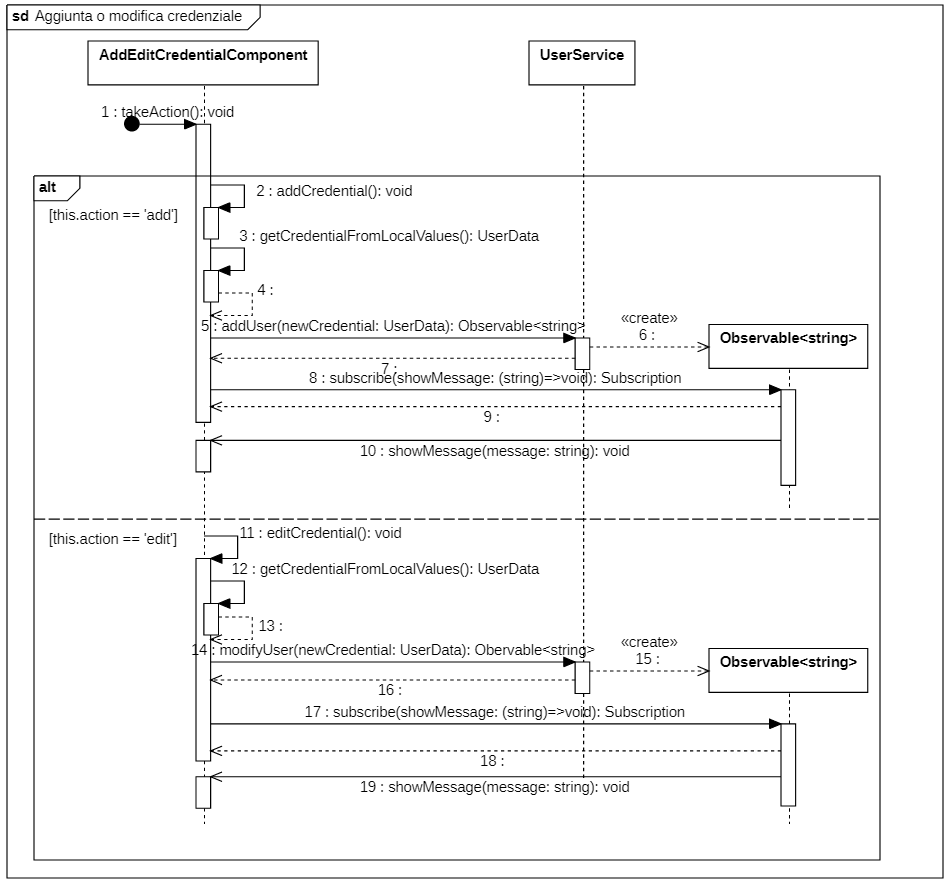
\includegraphics[width=18cm]{res/images/webapp-credenzialiAddEdit-diagrammaSequenza.png}
	\caption{Diagramma di sequenza per l'aggiunta e la modifica delle credenziali}
	\label{fig:DiagrammaSequenzaVisualizzazioneCredenziali}
\end{figure}
Il diagramma sovrastante rappresenta l'azione di aggiunta o modifica di una credenziale da parte di un'amministratore. L'evento è provocato dalla chiamata a \texttt{takeAction}, eseguita dall'utente tramite la pressione di un pulsante. Successivamente viene eseguita l'aggiunta (\texttt{addCredential}) o la modifica (\texttt{editCredential}) della credenziale definita dai valori inseriti precedentemente dall'utente. In entrambi i casi il componente invia i dati all'\texttt{UserService} e riceve un Observable, col quale può, tramite il metodo \texttt{subscribe}, inviare la chiamata al server e impostare una funzione di callback per gestirne la risposta.



